\mysection{Хакаем часы в Windows}

Иногда я устраиваю первоапрельские пранки для моих сотрудников.

Посмотрим, можем ли мы сделать что-то с часами в Windows?
Можем ли мы их заставить идти в обратную сторону?

Прежде всего, когда вы кликаете на часы/время в строке состояния (\emph{status bar}),\\
запускается модуль \emph{C:\textbackslash{}WINDOWS\textbackslash{}SYSTEM32\textbackslash{}TIMEDATE.CPL},
а это обычный \ac{PE}-файл.

Посмотрим, как отрисовываются стрелки?
Когда я открываю этот файл (из Windows 7) в Resource Hacker, здесь есть разные виды циферблата, но нет стрелок:

\begin{figure}[H]
\centering
\myincludegraphics{examples/timedate/reshack.png}
\caption{Resource Hacker}
\end{figure}

ОК, что мы знаем? Как рисовать стрелку часов? Они все начинаются в середине круга и заканчиваются на его границе.
Следовательно, нам нужно расчитать координаты точки на границе круга.
Из школьной математики мы можем вспомнить, что для рисования круга нужно использовать ф-ции синуса/косинуса, или
хотя бы квадратного корня.
Такого в \emph{TIMEDATE.CPL} нет, по крайней мере на первый взгляд.
Но, благодаря отладочным PDB-файлам от Microsoft, я могу найти ф-цию с названием \emph{CAnalogClock::DrawHand()}, которая
вызывает \emph{Gdiplus::Graphics::DrawLine()} минимум дважды.

Вот её код:

\lstinputlisting[style=customasmx86]{examples/timedate/1.lst}

\myindex{Windows!Win32!MulDiv()}
Мы можем увидеть что аргументы \emph{DrawLine()} зависят от результата ф-ции \emph{MulDiv()}
и таблицы \emph{table[]} (название дал я),
которая содержит 8-байтные элементы (посмотрите на второй операнд \INS{LEA}).

Что внутри table[]?

\lstinputlisting[style=customasmx86]{examples/timedate/2.lst}

Доступ к ней есть только из ф-ции \emph{DrawHand()}.
У ней 120 32-битных слов или 60 32-битных пар \dots подождите, 60?
Посмотрим ближе на эти значения.
Прежде всего, я затру нулями первые 6 пар или 12 32-битных слов, и затем я положу пропатченный \emph{TIMEDATE.CPL}
в \emph{C:\textbackslash{}WINDOWS\textbackslash{}SYSTEM32}.
(Вам, возможно, придется установить владельца файла *TIMEDATE.CPL* равным вашей первичной пользовательской учетной
записи (вместо \emph{TrustedInstaller}),
а также загрузиться в безопасном режиме с командной строкой, чтобы скопировать этот файл, который обычно залоченный.)

\begin{figure}[H]
\centering
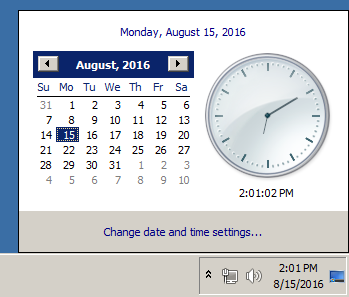
\includegraphics[width=0.5\textwidth]{examples/timedate/6_pairs_zeroed.png}
\caption{Attempt to run}
\end{figure}

Теперь, когда стрелка находится на 0..5 секундах/минутах, она невидимая! Хотя, противоположная (короткая) часть секундной
стрелки видима, и двигается.
Когда любая стрелка за пределами этой области, она видима, как обычно.

\myindex{Mathematica}
Посмотрим на эту таблицу при помощи Mathematica.
Я скопировал таблицу из \emph{TIMEDATE.CPL} в файл \emph{tbl} (480 байт).
Будем считать, что это знаковые значения, потому что половина элементов меньше нуля (0FFFFE0C1h, итд.).
Если бы эти значения были бы беззнаковыми, они были бы подозрительно большими.

\begin{lstlisting}[style=custommath]
In[]:= tbl = BinaryReadList["~/.../tbl", "Integer32"]

Out[]= {0, -7999, 836, -7956, 1663, -7825, 2472, -7608, 3253, -7308, 3999, \
-6928, 4702, -6472, 5353, -5945, 5945, -5353, 6472, -4702, 6928, \
-4000, 7308, -3253, 7608, -2472, 7825, -1663, 7956, -836, 8000, 0, \
7956, 836, 7825, 1663, 7608, 2472, 7308, 3253, 6928, 4000, 6472, \
4702, 5945, 5353, 5353, 5945, 4702, 6472, 3999, 6928, 3253, 7308, \
2472, 7608, 1663, 7825, 836, 7956, 0, 7999, -836, 7956, -1663, 7825, \
-2472, 7608, -3253, 7308, -4000, 6928, -4702, 6472, -5353, 5945, \
-5945, 5353, -6472, 4702, -6928, 3999, -7308, 3253, -7608, 2472, \
-7825, 1663, -7956, 836, -7999, 0, -7956, -836, -7825, -1663, -7608, \
-2472, -7308, -3253, -6928, -4000, -6472, -4702, -5945, -5353, -5353, \
-5945, -4702, -6472, -3999, -6928, -3253, -7308, -2472, -7608, -1663, \
-7825, -836, -7956}

In[]:= Length[tbl]
Out[]= 120
\end{lstlisting}

Будем считать два последовательно идущих 32-битных значения как пару:

\begin{lstlisting}[style=custommath]
In[]:= pairs = Partition[tbl, 2]
Out[]= {{0, -7999}, {836, -7956}, {1663, -7825}, {2472, -7608}, \
{3253, -7308}, {3999, -6928}, {4702, -6472}, {5353, -5945}, {5945, \
-5353}, {6472, -4702}, {6928, -4000}, {7308, -3253}, {7608, -2472}, \
{7825, -1663}, {7956, -836}, {8000, 0}, {7956, 836}, {7825, 
1663}, {7608, 2472}, {7308, 3253}, {6928, 4000}, {6472, 
4702}, {5945, 5353}, {5353, 5945}, {4702, 6472}, {3999, 
6928}, {3253, 7308}, {2472, 7608}, {1663, 7825}, {836, 7956}, {0, 
7999}, {-836, 7956}, {-1663, 7825}, {-2472, 7608}, {-3253, 
7308}, {-4000, 6928}, {-4702, 6472}, {-5353, 5945}, {-5945, 
5353}, {-6472, 4702}, {-6928, 3999}, {-7308, 3253}, {-7608, 
2472}, {-7825, 1663}, {-7956, 836}, {-7999, 
0}, {-7956, -836}, {-7825, -1663}, {-7608, -2472}, {-7308, -3253}, \
{-6928, -4000}, {-6472, -4702}, {-5945, -5353}, {-5353, -5945}, \
{-4702, -6472}, {-3999, -6928}, {-3253, -7308}, {-2472, -7608}, \
{-1663, -7825}, {-836, -7956}}

In[]:= Length[pairs]
Out[]= 60
\end{lstlisting}

Попробуем считать каждую пару как координату X/Y и нарисуем все 60 пар, а также первые 15 пар:

\begin{figure}[H]
\centering
\myincludegraphics{examples/timedate/math.png}
\caption{Mathematica}
\end{figure}

Ну теперь это кое-что!
Каждая пара это просто координата.
Первые 15 пар это координаты $\frac{1}{4}$ круга.

Видимо, разработчики в Microsoft расчитали все координаты предварительно и сохранили их в таблице.
\myindex{Memoization}
Это распространенная, хотя и немного олдскульная практика -- доступ к предвычисленным значениям в таблице быстрее, чем вызывать относительно медленные ф-ции
синуса/косинуса\footnote{Сегодня это называют \emph{memoization}}.
В наше время операции синуса/косинуса уже не такие \emph{дорогие}.

Теперь понятно, почему когда я затер первые 6 пар, стрелки были невидимы в этой области: на самом деле, стрелки рисовались,
просто их длина была нулевой, потому что стрелка начиналась в координатах 0:0, и там же и заканчивалась.

\subsubsection{Пранк (шутка)}

Учитывая всё это, можем ли мы заставить стрелки идти в обратную сторону?
На самом деле, это просто, нужно просто развернуть таблицу, так что каждая стрелка,
вместо отображения на месте нулевой секунды, рисовалась бы на месте 59-й секунды.

Когда-то давным давно я сделал патчер, в в самом начале 2000-х, для Windows 2000.
Трудно поверить, но он всё еще работает и для Windows 7, видимо, таблица с тех пор не менялась!

Исходник патчера: \url{\RepoURL/examples/timedate/time_pt.c}.

Теперь видно как стрелки идут назад:

\begin{figure}[H]
\centering
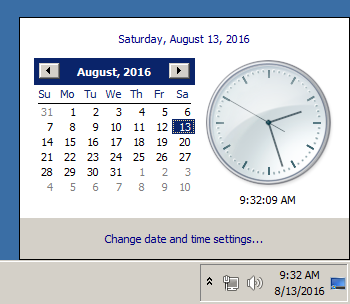
\includegraphics[width=0.5\textwidth]{examples/timedate/counterclockwise.png}
\caption{Now it works}
\end{figure}

В этой книге, конечно, нет анимации, но если присмотритесь, увидите, что на самом деле стрелки показывают корректное время,
но весь циферблат повернут вертикально, как если бы мы видели его изнутри часов.

\subsubsection{Утекшие исходники Windows 2000}

Так что я сделал патчер, потом утекли исходники Windows 2000 (я не могу заставить вас поверить мне, конечно).
Посмотрим на исходный код этой ф-ции и таблицы.\\
Нужный файл это \emph{win2k/private/shell/cpls/utc/clock.c}:

\begin{lstlisting}[style=customc]
//
//  Array containing the sine and cosine values for hand positions.
//
POINT rCircleTable[] =
{
    { 0,     -7999},
    { 836,   -7956},
    { 1663,  -7825},
    { 2472,  -7608},
    { 3253,  -7308},
...
    { -4702, -6472},
    { -3999, -6928},
    { -3253, -7308},
    { -2472, -7608},
    { -1663, -7825},
    { -836 , -7956},
};

////////////////////////////////////////////////////////////////////////////
//
//  DrawHand
//
//  Draws the hands of the clock.
//
////////////////////////////////////////////////////////////////////////////

void DrawHand(
    HDC hDC,
    int pos,
    HPEN hPen,
    int scale,
    int patMode,
    PCLOCKSTR np)
{
    LPPOINT lppt;
    int radius;

    MoveTo(hDC, np->clockCenter.x, np->clockCenter.y);
    radius = MulDiv(np->clockRadius, scale, 100);
    lppt = rCircleTable + pos;
    SetROP2(hDC, patMode);
    SelectObject(hDC, hPen);

    LineTo( hDC,
            np->clockCenter.x + MulDiv(lppt->x, radius, 8000),
            np->clockCenter.y + MulDiv(lppt->y, radius, 8000) );
}
\end{lstlisting}

Теперь всё ясно: координаты были предвычислены, как если бы циферблат был размером $2 \cdot 8000$,
а затем он масштабируется до радиуса текущего циферблата используя ф-цию \emph{MulDiv()}.

Структура POINT\footnote{\url{https://msdn.microsoft.com/en-us/library/windows/desktop/dd162805(v=vs.85).aspx}}
это структура из двух 32-битных значений, первое это \emph{x}, второе это \emph{y}.

